\documentclass[10pt,twocolumn]{article}

% ---------------------------------------------------------------------------
% Requirement-Aware Context Compression for Simulation-in-the-Loop Agents
% Self-contained arXiv-style two-column preprint. Builds with: tectonic main.tex
% ---------------------------------------------------------------------------

\usepackage[T1]{fontenc}
\usepackage{lmodern}
\usepackage[margin=0.85in]{geometry}
\usepackage{amsmath,amssymb}
\usepackage{booktabs}
\usepackage{graphicx}
\usepackage{xcolor}
\usepackage{microtype}
\usepackage{caption}
\usepackage{listings}
\usepackage{tikz}
\usepackage{pgfplots}
\pgfplotsset{compat=1.17}
\usetikzlibrary{arrows.meta,positioning,shapes.geometric}
\usepackage[colorlinks=true,linkcolor=blue!55!black,citecolor=blue!55!black,
            urlcolor=blue!55!black]{hyperref}

\definecolor{kw}{RGB}{30,80,170}
\definecolor{cm}{RGB}{110,120,130}
\definecolor{pass}{RGB}{20,130,60}
\definecolor{fail}{RGB}{190,40,40}
\definecolor{boxbg}{RGB}{246,247,249}

\lstdefinestyle{verd}{
  basicstyle=\ttfamily\scriptsize,
  backgroundcolor=\color{boxbg},
  frame=single, framesep=4pt, rulecolor=\color{black!15},
  breaklines=true, columns=fullflexible, keepspaces=true,
  xleftmargin=2pt, xrightmargin=2pt, aboveskip=6pt, belowskip=4pt,
  literate=
    {[PASS]}{{\textcolor{pass}{\bfseries[PASS]}}}{6}
    {[FAIL]}{{\textcolor{fail}{\bfseries[FAIL]}}}{6}
    {VERDICT:}{{\textcolor{kw}{\bfseries VERDICT:}}}{8},
}

\captionsetup{font=small,labelfont=bf}
\setlength{\parskip}{0pt}

% Ragged-right headings: no inter-word stretching, no ugly hyphenation in titles.
\usepackage{titlesec}
\titleformat{\section}{\normalfont\Large\bfseries\raggedright}{\thesection}{0.7em}{}
\titleformat{\subsection}{\normalfont\large\bfseries\raggedright}{\thesubsection}{0.6em}{}
\titlespacing*{\section}{0pt}{3.0ex plus 1ex minus .2ex}{1.5ex plus .2ex}
\titlespacing*{\subsection}{0pt}{2.4ex plus 1ex minus .2ex}{1.0ex plus .2ex}

% ---------------------------------------------------------------------------
\title{\bfseries Requirement-Aware Context Compression for\\
Simulation-in-the-Loop Agents}

\author{%
  Tazeem Mahashin\textsuperscript{1} \quad
  Ian Sun\textsuperscript{2} \quad
  Angela Choi\textsuperscript{3} \quad
  Matthew Han\textsuperscript{4}\\[3pt]
  \normalsize\textsuperscript{1}Rensselaer Polytechnic Institute \quad
  \textsuperscript{2}Massachusetts Institute of Technology\\
  \normalsize\textsuperscript{3}University of Pennsylvania \quad
  \textsuperscript{4}Georgia Institute of Technology%
}
\date{}

% ---------------------------------------------------------------------------
\begin{document}
\maketitle

\begin{abstract}
\noindent
Agentic loops that call a numerical simulator re-send the simulator's output to
the language model after every revision. For transient physical simulations this
output is a dense, multi-variable time series---hundreds of kilobytes of numeric
CSV per iteration---and it dominates the token cost of the loop because it
\emph{recurs} at every step. General-purpose text compressors barely help here:
they remove \emph{linguistic} redundancy, of which dense numeric output has
almost none. We argue that the right axis to compress along is not redundancy but
\emph{irrelevance}, and that what is relevant is defined by the downstream task's
own machine-checkable requirements. We present \emph{requirement-aware context
compression}: the agent runs the simulation at full fidelity, evaluates it
deterministically against the task's pass/fail predicates, and forwards only a
requirement-keyed verdict---one line per requirement, with the exact offending
value for any failure. On a real rocket-engine design loop of 14 iterations, this
compresses \mbox{2{,}379{,}129} tokens of raw simulator output to \mbox{3{,}065}
(a $99.87\%$ reduction) while preserving the decision-relevant signal byte-exact.
Measured in a byte-level compressor's own tokenizer, our pass takes a single
iteration from \mbox{198{,}358} to $433$ tokens ($99.78\%$), where that
compressor alone achieves $0.45\%$ and an LLM summary achieves $99.02\%$ but
\emph{drops} the failing value the design loop needs. The technique is
complementary to byte-level compression---which further shrinks our verdict by
$27\%$---and is domain-agnostic: it applies to any requirement-checked
time-series system.
\end{abstract}

% ===========================================================================
\section{Introduction}
\label{sec:intro}

A growing class of agents close a loop around a non-LLM tool: the model proposes
an artifact, a deterministic engine evaluates it, and the model revises. When the
engine is a physical simulator, the evaluation it returns is not a short status
code but a full \emph{transient time series}---every state variable of every
component at every timestep. In the design loop we study (Section~\ref{sec:problem}),
a single simulation emits on the order of $1.7\times10^{5}$ tokens of numeric CSV.
A naive agent forwards that output back to the model so it can revise; because the
loop iterates, this cost is paid \emph{again on every iteration}, and it is by a
wide margin the dominant term in the loop's token budget.

The obvious mitigation is to compress the tool output before sending it. But the
mainstream of context compression targets the wrong quantity. Prompt-compression
methods such as LLMLingua~\cite{jiang2023llmlingua,jiang2024longllmlingua} and
learned byte-level compressors exploit the fact that natural language is
statistically redundant: many tokens are predictable from their neighbors and can
be dropped or merged with little information loss. Dense numerical output has
almost none of this redundancy---each value is close to incompressible---so a
general compressor correctly leaves it nearly untouched. We confirm this directly:
a state-of-the-art hosted byte-level compressor reduces our raw simulator output by
only $0.45\%$ (Section~\ref{sec:results}).

Our central observation is that the simulator output is nonetheless \emph{enormously}
compressible, just not along the redundancy axis. It is compressible along the axis
of \emph{relevance}: of the hundreds of thousands of numbers in the time series,
the next design revision depends on only a handful---precisely those that the task's
acceptance criteria test. Crucially, in a requirement-driven loop those criteria are
already written down, as machine-checkable predicates over the simulator's output
fields. We can therefore condition the compressor on them.

We call this \emph{requirement-aware context compression}. Rather than paraphrase
the raw output, the agent (i)~runs the simulation at full fidelity, (ii)~evaluates
the task's predicates against the complete time series in deterministic code, and
(iii)~forwards only a \emph{requirement-keyed verdict}: one line per requirement,
marked pass or fail, annotated for each failure with the exact actual value, the
statistic and field it came from, and the threshold it violated. Everything that
does not bear on a requirement is dropped. What survives is exactly the signal the
model needs to revise, and its size is $O(\text{\#requirements})$---independent of
the length of the time series.

\paragraph{Contributions.}
\begin{itemize}\setlength\itemsep{1pt}
\item We identify \emph{relevance}, not redundancy, as the compressible axis of
numeric tool output in requirement-driven agent loops, and formalize a compression
operator conditioned on the task's machine-checkable requirements
(Section~\ref{sec:method}).
\item We give a domain-agnostic kernel,
\texttt{compress\_tabular\_context}, that applies to any list-of-rows checked
against \texttt{(field, stat, op, value)} predicates---logs versus SLOs, metrics
versus thresholds, benchmark output versus targets---and a \texttt{protect()}
discipline that lets the verdict be safely stacked under a lossy byte-level
compressor while keeping every critical number byte-exact.
\item On a real 14-iteration rocket-engine design loop we measure a $99.87\%$
reduction ($2{,}379{,}129\!\to\!3{,}065$ tokens). In a head-to-head using a
byte-level compressor's own tokenizer, our verdict reaches $99.78\%$
($198{,}358\!\to\!433$) where the byte-level compressor reaches $0.45\%$ and an
LLM summary reaches $99.02\%$ but discards the decision-relevant value
(Section~\ref{sec:results}).
\item We show the two approaches are \emph{complementary}: a byte-level
compressor shaves a further $27\%$ off our already-tiny verdict, so the right
architecture applies requirement-aware compression to the heavy numeric
tool-output and byte-level compression to the static prose prefix.
\end{itemize}

% ===========================================================================
\section{Related Work}
\label{sec:related}

\paragraph{Prompt and context compression.}
LLMLingua and LongLLMLingua~\cite{jiang2023llmlingua,jiang2024longllmlingua}
compress prompts by deleting low-information tokens under a small language model,
exploiting the redundancy of natural language; Selective
Context~\cite{li2023selective} prunes by self-information. These operate on prose
and are task-agnostic---they do not know what the reader will do with the text.
Our method is orthogonal: it compresses a structured numeric artifact by
conditioning on the consumer's explicit acceptance test, and it composes with a
byte-level prose compressor rather than competing with it
(Section~\ref{sec:results}).

\paragraph{Retrieval and summarization.}
Retrieval-augmented generation~\cite{lewis2020rag} and abstractive summarization
reduce what reaches the model by selecting or rewriting passages. Both are lossy in
an uncontrolled way for our setting: a summarizer asked to condense a dense numeric
table has no principled basis for which of the thousands of values to keep, and---as
we measure in Section~\ref{sec:results}---spends its budget on salient-looking
prose while silently dropping the one value the loop tests against. Requirement-aware
compression makes that selection aligned with the downstream check \emph{by
construction}.

\paragraph{Tool-using and self-refining agents.}
ReAct~\cite{yao2023react}, Reflexion~\cite{shinn2023reflexion}, and
Toolformer~\cite{schick2023toolformer} interleave model reasoning with external
tool calls and feed tool observations back into context. Our work targets the cost
of that feedback channel when the tool is a high-volume numerical simulator, and
replaces the raw observation with a task-conditioned verdict. The idea of returning
a structured judgement rather than raw output is related to verifier- and
checker-in-the-loop training~\cite{cobbe2021verifiers}, but we apply it as an
\emph{inference-time context-compression} mechanism.

% ===========================================================================
\section{Problem Setting}
\label{sec:problem}

\paragraph{The loop.}
We study an LLM-in-the-loop design system for rocket propellant feed systems. The
loop is
\[\textstyle
\text{spec}\to\underbrace{\text{LLM design}}_{\text{revise}}\to\text{sim}
\to\text{verdict}\to\cdots
\]
A \emph{spec} fixes the design target and carries a set of machine-checkable
\emph{checks}. The model emits a network of nodes (tanks, engine) and connections
(feed lines with effective areas), the simulator integrates the transient fluid
network, and the resulting state is evaluated against the checks to decide whether
to stop or revise.

\paragraph{What the simulator emits.}
The simulator produces two CSV tables per run, \texttt{nodes.csv} and
\texttt{connections.csv}, holding every node/connection $\times$ every field
(pressure, temperature, density, internal energy, mass flow, mixture ratio,
thrust, \dots) $\times$ every timestep. Runs reach tens of thousands of rows and
hundreds of kilobytes. At a conservative 4 characters/token this is
$\approx\!1.7\times10^{5}$ tokens per iteration; measured in a production byte-level
tokenizer the same output is $\approx\!1.98\times10^{5}$ tokens, because dense
numerics tokenize \emph{more} finely than prose (Section~\ref{sec:results}).

\paragraph{Cost model.}
Let $R$ be the per-iteration size of the raw simulator output and $V$ the size of
the compressed verdict, with $V\ll R$. A loop that forwards raw output pays $\Theta(R)$
of \emph{recurring} input per iteration on top of the conversation; over $N$
iterations the cumulative simulator-output cost is $\Theta(NR)$, and if the
transcript is replayed it grows as $\Theta(N^2 R)$. Requirement-aware compression
replaces $R$ with $V$, making the recurring term $\Theta(V)$ with
$V=O(\text{\#requirements})$, independent of the time-series length. Because $R$ is
nearly three orders of magnitude larger than $V$ ($R/V\approx\!780$ here), this term
effectively disappears (Figure~\ref{fig:cost}).

% ===========================================================================
\section{Method}
\label{sec:method}

\subsection{Requirement-aware compression operator}

Let the simulation produce a record sequence $X=(x_1,\dots,x_T)$, where each $x_t$
maps field names to values at timestep $t$. Let the task carry requirements
$Q=\{q_1,\dots,q_m\}$, each a predicate
\[
q_i=\bigl(f_i,\; s_i,\; \triangleright_i,\; \theta_i,\; d_i\bigr),
\]
with field $f_i$, statistic
$s_i\in\{\textsf{final},\textsf{first},\textsf{min},\textsf{max},\textsf{mean},\textsf{count}\}$,
comparison operator $\triangleright_i\in\{\ge,\le,>,<,=,\ne\}$, threshold $\theta_i$,
and human description $d_i$. Define the column aggregator
\[
A(X,f,s)=s\bigl(\langle x_t[f]\rangle_{t:\,x_t[f]\neq\bot}\bigr),
\]
i.e.\ apply statistic $s$ to the non-missing values of field $f$ across all
timesteps. The compression operator is
\[
\mathcal{C}(X,Q)=\Bigl\langle \bigl(\mathbb{1}[a_i \triangleright_i \theta_i],\,
d_i,\, \rho_i\bigr)\Bigr\rangle_{i=1}^{m},\; a_i=A(X,f_i,s_i),
\]
where the per-requirement payload is
\[
\rho_i=\begin{cases}
\varnothing & \text{if } a_i \triangleright_i \theta_i \text{ (pass)},\\[2pt]
\bigl(s_i(f_i),\,\triangleright_i,\,\theta_i,\,a_i\bigr) & \text{otherwise (fail)}.
\end{cases}
\]
Passing requirements contribute only a tag; failing ones additionally carry the
exact actual value $a_i$ and the violated predicate, so the model sees precisely
\emph{what} failed and \emph{by how much}. The serialized verdict has length
$O(m)$ and is independent of $T$. An example produced by the real loop is shown in
Listing~\ref{lst:verdict}.

\begin{lstlisting}[style=verd,caption={A real verdict for one iteration of the
\texttt{lox\_methane\_engine} spec (8 checks). The raw simulator output for this
same iteration is $\approx\!198\mathrm{k}$ tokens; this verdict is $433$.},
label={lst:verdict},escapechar=!]
VERDICT: 5/8 checks passed

[PASS] ran: Simulation runs without crash.
[PASS] flow_happens: Propellant actually flows.
[FAIL] thrust_min: End-of-burn thrust >= 1500 N.
   expected >= 1500.0; actual=1136.79
   (engine.thrust.final=1136.79)
[PASS] thrust_max: End-of-burn thrust <= 2500 N.
[PASS] mr_min: Mixture ratio >= 2.8.
[PASS] mr_max: Mixture ratio <= 3.6.
[FAIL] chamber_pressure: P_c >= 1.2 MPa.
   expected >= 1200000.0; actual=970428
[FAIL] isp: Specific impulse >= 195 s.
   expected >= 195.0; actual=193.132

TARGETED REVISION ADVICE:
 - Thrust low (1137 N vs 1500). Increase ox
   and fuel CdA together by ~1.52x.
\end{lstlisting}

\subsection{Why the verdict preserves the signal}

The verdict is lossy with respect to the raw time series but \emph{lossless with
respect to the decision}: by construction it contains every quantity any
requirement tests, at full precision, plus the sign and magnitude of each
violation. The model never has to parse a $10^5$-token table to recover the handful
of numbers that matter; it receives them directly, already attributed to the check
they break. This is why the compressed representation is not merely smaller but a
\emph{better} input: it removes noise, not signal (Section~\ref{sec:results}).

\subsection{Domain-agnostic kernel}

Nothing above is rocket-specific. The same operator applies to any list-of-rows
checked against requirements. We expose it as
\texttt{compress\_tabular\_context(records, requirements)}, taking generic rows and
a requirement set of \texttt{(field, stat, op, value)} predicates and emitting the
same requirement-keyed verdict. A 5{,}000-row request-latency log checked against a
single SLO (\textsf{max}(\texttt{latency\_ms}) $<500$) compresses to a one-line
verdict with the offending maximum---$>\!95\%$ reduction versus serializing the
log---by exactly the mechanism used for the simulator.

\subsection{Composition with byte-level compression}
\label{sec:protect}

Requirement-aware compression and byte-level prose compression are orthogonal and
compose. We apply the former to the heavy numeric tool-output and the latter to the
static prose prefix (system prompt, spec, seed design). Because a learned
byte-level compressor is lossy, we wrap every critical span---spec JSON, seed
design, and the verdict's numerals---in a \texttt{protect()} fence that instructs
the compressor to pass those bytes through verbatim. This lets us stack a hosted
compressor on top of the verdict without risking corruption of a value the loop
depends on. Empirically the byte-level pass removes a further $27\%$ of the
already-tiny verdict (Section~\ref{sec:results}).

% ===========================================================================
\section{Experimental Setup}
\label{sec:setup}

\paragraph{Workload.}
We measure on three real multi-iteration design runs from the rocketcursor loop:
\texttt{lox\_methane\_engine} (a LOX/methane engine, 8 checks, 6 iterations),
\texttt{nitrogen\_blowdown\_vent} (a blowdown vent, 2 iterations), and
\texttt{pressure\_window\_blowdown} (9 checks, 6 iterations)---14 iterations in
total. For each iteration we have the simulator's raw \texttt{nodes.csv} and
\texttt{connections.csv} and the recorded result the verdict is computed from.

\paragraph{What we compare.}
For every iteration we compare the bytes a naive loop would forward---the raw CSV
concatenation---against the verdict our loop actually sends. The savings are
\emph{recurring}: the raw cost is paid every iteration of a multi-step loop.

\paragraph{Tokenization.}
Two regimes appear, and we keep them distinct. (i)~For the aggregate sweep we use a
tokenizer-agnostic estimate of 4 characters/token; the compression \emph{ratio} is
robust to the exact tokenizer. (ii)~For the head-to-head against a byte-level
compressor we report that compressor's \emph{own} tokenizer counts, which is the
apples-to-apples basis for comparing against it---and which counts the raw output
\emph{higher} ($1.98\times10^{5}$) than the 4-char estimate ($1.70\times10^{5}$),
because dense numerics tokenize finely. Our reported head-to-head reduction is thus
if anything conservative.

\paragraph{Baselines.}
We compare against (a)~a hosted byte-level compressor (\texttt{bear-2}) run on the
raw output at low and maximum aggressiveness, and (b)~an LLM summarization baseline:
a frontier model (\texttt{claude-sonnet-4-6}) prompted to summarize the raw CSV for
the design model while ``preserving every engineering quantity that could matter for
a pass/fail decision.'' All numbers are produced by
\texttt{python -m loop.compression\_benchmark} and the accompanying scripts; raw
outputs and the saved \texttt{benchmark.json} accompany the code.

% ===========================================================================
\section{Results}
\label{sec:results}

\subsection{Aggregate reduction}

Table~\ref{tab:agg} reports the per-run and total reduction across all 14
iterations. The loop's $2{,}379{,}129$ tokens of raw simulator output compress to
$3{,}065$---a $99.87\%$ reduction, averaging $\approx\!1.7\times10^{5}$ raw down to
$\approx\!220$ sent per iteration.

\begin{table}[t]
\centering\small
\caption{Requirement-aware reduction over 14 real iterations (4-char/token
estimate). \emph{sent} is the verdict actually forwarded to the model.}
\label{tab:agg}
\setlength{\tabcolsep}{4pt}
\resizebox{\columnwidth}{!}{%
\begin{tabular}{lrrrr}
\toprule
spec & iters & raw tok & sent tok & reduction\\
\midrule
\texttt{lox\_methane\_engine}     & 6 & 334{,}882   & 1{,}491 & 99.55\%\\
\texttt{nitrogen\_blowdown\_vent} & 2 & 1{,}286{,}112 & 226   & 99.98\%\\
\texttt{pressure\_window\_blowdown}& 6 & 758{,}135  & 1{,}348 & 99.82\%\\
\midrule
\textbf{Total} & \textbf{14} & \textbf{2{,}379{,}129} & \textbf{3{,}065} & \textbf{99.87\%}\\
\bottomrule
\end{tabular}}
\end{table}

\begin{figure}[t]
\centering
\resizebox{\columnwidth}{!}{%
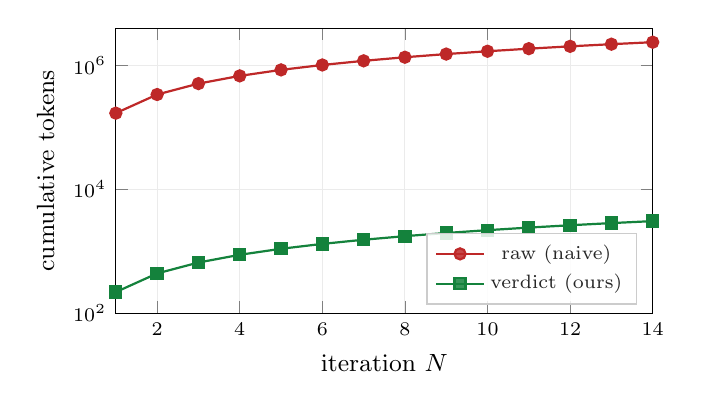
\begin{tikzpicture}
\begin{axis}[
  width=8.4cm, height=5.2cm,
  xlabel={iteration $N$}, ylabel={cumulative tokens},
  ymode=log, log basis y=10,
  xmin=1, xmax=14, ymin=100, ymax=4e6,
  xtick={2,4,6,8,10,12,14},
  legend pos=south east, legend style={font=\scriptsize,fill=white,fill opacity=0.85,draw=black!20},
  tick label style={font=\scriptsize}, label style={font=\small},
  grid=both, grid style={black!8},
]
\addplot[mark=*,thick,fail] coordinates {
 (1,169938)(2,339876)(3,509814)(4,679752)(5,849690)(6,1019628)
 (7,1189566)(8,1359504)(9,1529442)(10,1699380)(11,1869318)(12,2039256)(13,2209194)(14,2379132)};
\addlegendentry{raw (naive)}
\addplot[mark=square*,thick,pass] coordinates {
 (1,219)(2,438)(3,657)(4,876)(5,1095)(6,1314)(7,1533)(8,1752)
 (9,1971)(10,2190)(11,2409)(12,2628)(13,2847)(14,3065)};
\addlegendentry{verdict (ours)}
\end{axis}
\end{tikzpicture}}
\caption{Cumulative simulator-feedback tokens over the 14-iteration workload
(log scale). The recurring raw-output term ($\approx\!1.7\times10^5$/iter) is
nearly three orders of magnitude larger than the verdict ($\approx\!220$/iter).}
\label{fig:cost}
\end{figure}

\subsection{Head-to-head vs.\ byte-level and summarization}

Table~\ref{tab:h2h} compares, on a single iteration and in the byte-level
compressor's own tokenizer, four ways of reducing the raw output. The general
byte-level compressor is near-inert on dense numerics ($0.45\%$ at maximum
aggressiveness): there is little linguistic redundancy to exploit. The LLM
summarization baseline does shrink the output ($99.02\%$), but it is both
$4.5\times$ larger than our verdict \emph{and} lossy on the decision: in our run it
spent its budget describing tank states and never emitted the end-of-burn engine
thrust ($1136.79$~N) that the spec's binding \texttt{thrust\_min} check tests---the
single most decision-relevant number is simply absent. Requirement-aware compression reaches
$99.78\%$ ($458\times$) and preserves that value byte-exact.

\begin{table}[t]
\centering\small
\caption{One iteration of \texttt{lox\_methane\_engine}, measured in the
byte-level compressor's own tokenizer. ``keeps actual?'' is whether the
decision-relevant failing value ($1136.79$~N) survives.}
\label{tab:h2h}
\setlength{\tabcolsep}{4pt}
\resizebox{\columnwidth}{!}{%
\begin{tabular}{lrr c}
\toprule
method & raw$\to$out & reduction & keeps actual?\\
\midrule
\textbf{Ours (req.-aware)}      & 198{,}358$\to$\textbf{433}    & \textbf{99.78\%} & \textcolor{pass}{yes}\\
\texttt{bear-2}, aggr.\ 0.5     & 198{,}358$\to$198{,}356      & 0.00\%  & ---\\
\texttt{bear-2}, aggr.\ 0.9     & 198{,}358$\to$197{,}466      & 0.45\%  & ---\\
LLM summary                     & 198{,}358$\to$1{,}948        & 99.02\% & \textcolor{fail}{no}\\
\bottomrule
\end{tabular}}
\end{table}

\subsection{The methods compose}

Requirement-aware compression and byte-level compression remove different things, so
they stack. Running the hosted \texttt{bear-2} compressor \emph{on our verdict}
shrinks it a further $27\%$ ($433\to315$ tokens). The intended architecture
therefore uses requirement-aware compression for the heavy numeric tool-output and
byte-level compression for the static prose prefix, with \texttt{protect()} fences
(Section~\ref{sec:protect}) keeping every critical numeral byte-exact through the
lossy pass.

\subsection{Quality of the compressed signal}

The compression preserves the loop's ability to revise. Acting only on the
$\approx\!220$-token verdict---never on the raw time series---the model makes
targeted, attributable design changes: on \texttt{lox\_methane\_engine} it improves
from $5/8$ to $6/8$ passing checks while adjusting exactly the feed areas the
verdict's thrust failure points to (Listing~\ref{lst:verdict}). The verdict carries
the failing magnitude and a derived revision direction, so the model is never asked
to recover a control signal by parsing $10^5$ tokens of CSV. Consistent with the
summarization result above, this supports the claim that the verdict is a
\emph{better} input than the raw output, not merely a cheaper one. We do not claim
the loop reaches all-pass on every spec within the recorded budget; our claim is on
the fidelity and cost of the feedback channel, which the data above establish.

% ===========================================================================
\section{Discussion}
\label{sec:discuss}

\paragraph{Why requirement-awareness is the right axis.}
The three baselines in Table~\ref{tab:h2h} cleanly separate two compressible axes.
Byte-level compression targets redundancy and is near-inert here because numeric
output has none. Summarization targets salience but has no principled link to the
downstream decision, so it discards the tested value. Requirement-aware compression
targets relevance and grounds it in the task's own predicates, which both bounds the
output size by the number of requirements and guarantees the tested quantities
survive. The win is not a better squeeze of the same information; it is compressing
a different, smaller object---the decision---rather than the data.

\paragraph{Generality.}
The operator needs only (i)~a high-volume tabular/time-series tool output and
(ii)~machine-checkable requirements over its fields. Both are common far outside
rocketry: service logs against SLOs, monitoring metrics against alert thresholds,
financial series against risk limits, CI/benchmark output against regression
targets. In each case the same \texttt{(field, stat, op, value)} kernel applies.

\paragraph{Limitations.}
The verdict carries only what the requirements ask for; a quantity that is
decision-relevant but \emph{unchecked} will be dropped, so the method is only as
complete as the requirement set. This is a feature for cost and a risk for
discovery: exploratory analysis that needs the full series should bypass the
compressor. The aggregator currently supports scalar statistics over fields;
requirements that depend on temporal \emph{shape} (e.g.\ overshoot duration) require
richer statistics, which the same framework admits as additional \texttt{stat}
kinds. Finally, our quality evidence is the loop's targeted revision behavior and a
single measured summarization comparison; a larger controlled study of downstream
solve rate under matched budgets is future work.

% ===========================================================================
\section{Conclusion}
\label{sec:conclusion}

Numeric tool output in agent loops is barely compressible along the redundancy axis
that general compressors exploit, yet it is extraordinarily compressible along the
axis of relevance---and in requirement-driven loops the relevant quantities are
already specified as machine-checkable predicates. Conditioning the compressor on
those predicates turns a recurring $10^5$-token feedback channel into a
$\sim\!10^2$-token verdict that is lossless with respect to the decision, preserves
critical values byte-exact, and composes with byte-level compression of the prose
prefix. Across a real 14-iteration design loop this is a $99.87\%$ reduction with no
loss of---indeed an improvement in---the signal the model revises against. The
mechanism is domain-agnostic, and we expect it to apply wherever an agent loops
around a high-volume, requirement-checked tool.

\paragraph{Reproducibility.}
The compressor (\texttt{loop/compression.py}), the deterministic evaluator
(\texttt{loop/evaluator.py}), the benchmark
(\texttt{loop/compression\_benchmark.py}, including the \texttt{--ttc} head-to-head),
and the saved results (\texttt{results/compression/benchmark.json}) accompany this
paper. The aggregate table reproduces with
\texttt{python -m loop.compression\_benchmark}; the head-to-head and summarization
baselines require API keys for the respective hosted services.

% ===========================================================================
\begin{thebibliography}{99}
\small
\bibitem{jiang2023llmlingua} H.~Jiang, Q.~Wu, C.-Y.~Lin, Y.~Yang, and L.~Qiu.
LLMLingua: Compressing Prompts for Accelerated Inference of Large Language Models.
\emph{EMNLP}, 2023.

\bibitem{jiang2024longllmlingua} H.~Jiang, Q.~Wu, X.~Luo, D.~Li, C.-Y.~Lin,
Y.~Yang, and L.~Qiu. LongLLMLingua: Accelerating and Enhancing LLMs in Long Context
Scenarios via Prompt Compression. \emph{ACL}, 2024.

\bibitem{li2023selective} Y.~Li, B.~Dong, F.~Guerin, and C.~Lin. Compressing
Context to Enhance Inference Efficiency of Large Language Models. \emph{EMNLP},
2023.

\bibitem{lewis2020rag} P.~Lewis et al. Retrieval-Augmented Generation for
Knowledge-Intensive NLP Tasks. \emph{NeurIPS}, 2020.

\bibitem{yao2023react} S.~Yao, J.~Zhao, D.~Yu, N.~Du, I.~Shafran, K.~Narasimhan,
and Y.~Cao. ReAct: Synergizing Reasoning and Acting in Language Models.
\emph{ICLR}, 2023.

\bibitem{shinn2023reflexion} N.~Shinn, F.~Cassano, E.~Berman, A.~Gopinath,
K.~Narasimhan, and S.~Yao. Reflexion: Language Agents with Verbal Reinforcement
Learning. \emph{NeurIPS}, 2023.

\bibitem{schick2023toolformer} T.~Schick, J.~Dwivedi-Yu, R.~Dess\`i, R.~Raileanu,
M.~Lomeli, L.~Zettlemoyer, N.~Cancedda, and T.~Scialom. Toolformer: Language Models
Can Teach Themselves to Use Tools. \emph{NeurIPS}, 2023.

\bibitem{cobbe2021verifiers} K.~Cobbe et al. Training Verifiers to Solve Math Word
Problems. \emph{arXiv:2110.14168}, 2021.
\end{thebibliography}

\end{document}
